\documentclass{beamer}
\usepackage{ragged2e}
\usepackage{CJKutf8}
\usepackage{tikz}
\setbeamertemplate{theorems}[numbered]
\justifying\let\raggedright\justifying
\begin{document}
\begin{CJK*}{UTF8}{gbsn}

  \newtheorem*{Thm}{定理}
  \newtheorem{Thm1}{定理}

\theoremstyle{definition}
\newtheorem{Def}{定义}
\theoremstyle{example}
\newtheorem*{Ex}{例:}
\newtheorem*{Exercise}{习题}
\newtheorem{Exercise1}{习题}

\date{}
\author{陈建文}
\title{习题讲解}
\begin{frame}
  \titlepage
\end{frame}


\begin{frame}
  \frametitle{数学归纳法I}

  \begin{Thm} 
  $\forall n P(n)$   
\end{Thm}\pause
\begin{proof}[证明]
  用数学归纳法证明,施归纳于$n$。\pause

  (1)当$n=0$时$P(n)$成立。\pause

  (2)假设当$n=k(k\geq 1)$时$P(n)$成立,往证当$n=k+1$时$P(n)$也成立。
\end{proof}
\pause
(1)$P(0)$\pause

(2)$P(k)\to P(k+1)$

\pause
$P(0)$ \pause $P(1)$ \pause  $P(2)$ \pause $\cdots$
  
\end{frame}

\begin{frame}
    \begin{Thm}
  设树$T$有$p$个顶点,$q$条边,则$q = p-1$。
  \end{Thm}\pause
\centering
  \begin{minipage}{0.24\linewidth}
    \centering
    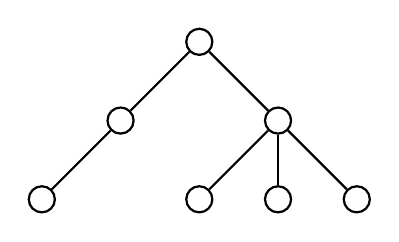
\begin{tikzpicture}[auto,
    specification/.style ={circle, draw, thick}]
   \node[specification] (A)  at (0,0)  {};
   \node[specification] (B)  at (-1,-1)  {};
   \node[specification] (C)  at (1,-1)  {};
   \node[specification] (D)  at (-2,-2)  {};
   \node[specification] (E)  at (0,-2)  {};
   \node[specification] (F)  at (1,-2)  {};
   \node[specification] (G)  at (2,-2)  {};

   \draw[thick] (A) to  (B);
   \draw[thick] (A) to (C);
   \draw[thick] (B) to (D);
   \draw[thick] (C) to (E);
   \draw[thick] (C) to (F);
   \draw[thick] (C) to (G);   
 \end{tikzpicture}
\end{minipage}
\end{frame}
\begin{frame}
    \begin{Thm}
  设树$T$有$p$个顶点,$q$条边,则$q = p-1$。
  \end{Thm}
\centering
  \begin{minipage}{0.24\linewidth}
    \centering
    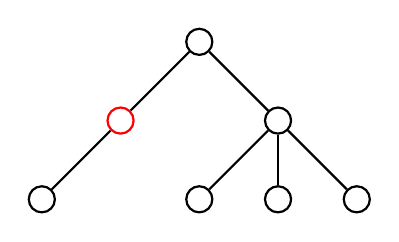
\begin{tikzpicture}[auto,
    specification/.style ={circle, draw, thick}]
   \node[specification] (A)  at (0,0)  {};
   \node[specification,red] (B)  at (-1,-1)  {};
   \node[specification] (C)  at (1,-1)  {};
   \node[specification] (D)  at (-2,-2)  {};
   \node[specification] (E)  at (0,-2)  {};
   \node[specification] (F)  at (1,-2)  {};
   \node[specification] (G)  at (2,-2)  {};

   \draw[thick] (A) to  (B);
   \draw[thick] (A) to (C);
   \draw[thick] (B) to (D);
   \draw[thick] (C) to (E);
   \draw[thick] (C) to (F);
   \draw[thick] (C) to (G);   
 \end{tikzpicture}
\end{minipage}
\end{frame}
\begin{frame}
    \begin{Thm}
  设树$T$有$p$个顶点,$q$条边,则$q = p-1$。
  \end{Thm}
\centering
  \begin{minipage}{0.24\linewidth}
    \centering
    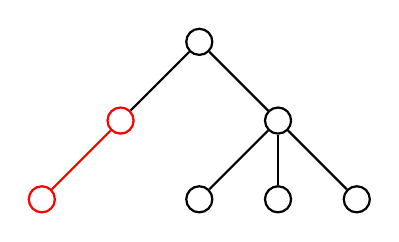
\begin{tikzpicture}[auto,
    specification/.style ={circle, draw, thick}]
   \node[specification] (A)  at (0,0)  {};
   \node[specification,red] (B)  at (-1,-1)  {};
   \node[specification] (C)  at (1,-1)  {};
   \node[specification,red] (D)  at (-2,-2)  {};
   \node[specification] (E)  at (0,-2)  {};
   \node[specification] (F)  at (1,-2)  {};
   \node[specification] (G)  at (2,-2)  {};

   \draw[thick] (A) to  (B);
   \draw[thick] (A) to (C);
   \draw[thick,red] (B) to (D);
   \draw[thick] (C) to (E);
   \draw[thick] (C) to (F);
   \draw[thick] (C) to (G);   
 \end{tikzpicture}
\end{minipage}
\end{frame}
\begin{frame}
    \begin{Thm}
  设树$T$有$p$个顶点,$q$条边,则$q = p-1$。
  \end{Thm}
\centering
  \begin{minipage}{0.24\linewidth}
    \centering
    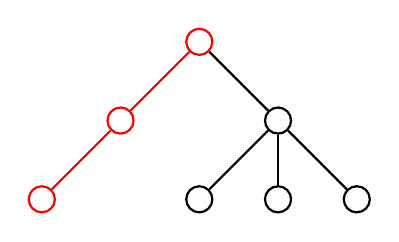
\begin{tikzpicture}[auto,
    specification/.style ={circle, draw, thick}]
   \node[specification,red] (A)  at (0,0)  {};
   \node[specification,red] (B)  at (-1,-1)  {};
   \node[specification] (C)  at (1,-1)  {};
   \node[specification,red] (D)  at (-2,-2)  {};
   \node[specification] (E)  at (0,-2)  {};
   \node[specification] (F)  at (1,-2)  {};
   \node[specification] (G)  at (2,-2)  {};

   \draw[thick,red] (A) to  (B);
   \draw[thick] (A) to (C);
   \draw[thick,red] (B) to (D);
   \draw[thick] (C) to (E);
   \draw[thick] (C) to (F);
   \draw[thick] (C) to (G);   
 \end{tikzpicture}
\end{minipage}
\end{frame}
\begin{frame}
    \begin{Thm}
  设树$T$有$p$个顶点,$q$条边,则$q = p-1$。
  \end{Thm}
\centering
  \begin{minipage}{0.24\linewidth}
    \centering
    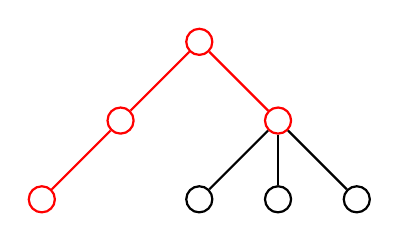
\begin{tikzpicture}[auto,
    specification/.style ={circle, draw, thick}]
   \node[specification,red] (A)  at (0,0)  {};
   \node[specification,red] (B)  at (-1,-1)  {};
   \node[specification,red] (C)  at (1,-1)  {};
   \node[specification,red] (D)  at (-2,-2)  {};
   \node[specification] (E)  at (0,-2)  {};
   \node[specification] (F)  at (1,-2)  {};
   \node[specification] (G)  at (2,-2)  {};

   \draw[thick,red] (A) to  (B);
   \draw[thick,red] (A) to (C);
   \draw[thick,red] (B) to (D);
   \draw[thick] (C) to (E);
   \draw[thick] (C) to (F);
   \draw[thick] (C) to (G);   
 \end{tikzpicture}
\end{minipage}
\end{frame}
\begin{frame}
    \begin{Thm}
  设树$T$有$p$个顶点,$q$条边,则$q = p-1$。
  \end{Thm}
\centering
  \begin{minipage}{0.24\linewidth}
    \centering
    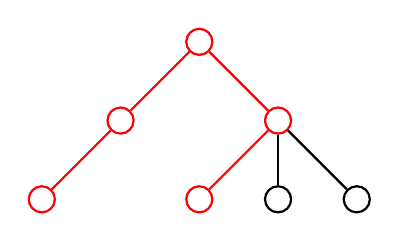
\begin{tikzpicture}[auto,
    specification/.style ={circle, draw, thick}]
   \node[specification,red] (A)  at (0,0)  {};
   \node[specification,red] (B)  at (-1,-1)  {};
   \node[specification,red] (C)  at (1,-1)  {};
   \node[specification,red] (D)  at (-2,-2)  {};
   \node[specification,red] (E)  at (0,-2)  {};
   \node[specification] (F)  at (1,-2)  {};
   \node[specification] (G)  at (2,-2)  {};

   \draw[thick,red] (A) to  (B);
   \draw[thick,red] (A) to (C);
   \draw[thick,red] (B) to (D);
   \draw[thick,red] (C) to (E);
   \draw[thick] (C) to (F);
   \draw[thick] (C) to (G);   
 \end{tikzpicture}
\end{minipage}
\end{frame}
\begin{frame}
    \begin{Thm}
  设树$T$有$p$个顶点,$q$条边,则$q = p-1$。
  \end{Thm}
\centering
  \begin{minipage}{0.24\linewidth}
    \centering
    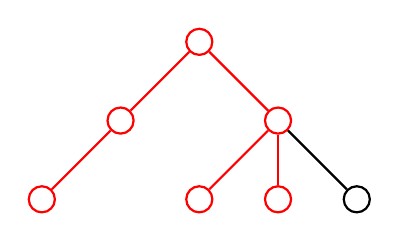
\begin{tikzpicture}[auto,
    specification/.style ={circle, draw, thick}]
   \node[specification,red] (A)  at (0,0)  {};
   \node[specification,red] (B)  at (-1,-1)  {};
   \node[specification,red] (C)  at (1,-1)  {};
   \node[specification,red] (D)  at (-2,-2)  {};
   \node[specification,red] (E)  at (0,-2)  {};
   \node[specification,red] (F)  at (1,-2)  {};
   \node[specification] (G)  at (2,-2)  {};

   \draw[thick,red] (A) to  (B);
   \draw[thick,red] (A) to (C);
   \draw[thick,red] (B) to (D);
   \draw[thick,red] (C) to (E);
   \draw[thick,red] (C) to (F);
   \draw[thick] (C) to (G);   
 \end{tikzpicture}
\end{minipage}
\end{frame}
\begin{frame}
    \begin{Thm}
  设树$T$有$p$个顶点,$q$条边,则$q = p-1$。
  \end{Thm}
\centering
  \begin{minipage}{0.24\linewidth}
    \centering
    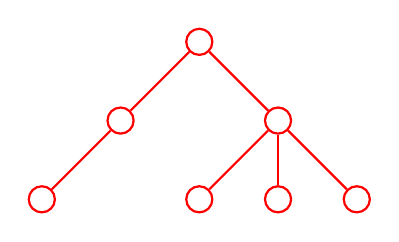
\begin{tikzpicture}[auto,
    specification/.style ={circle, draw, thick}]
   \node[specification,red] (A)  at (0,0)  {};
   \node[specification,red] (B)  at (-1,-1)  {};
   \node[specification,red] (C)  at (1,-1)  {};
   \node[specification,red] (D)  at (-2,-2)  {};
   \node[specification,red] (E)  at (0,-2)  {};
   \node[specification,red] (F)  at (1,-2)  {};
   \node[specification,red] (G)  at (2,-2)  {};

   \draw[thick,red] (A) to  (B);
   \draw[thick,red] (A) to (C);
   \draw[thick,red] (B) to (D);
   \draw[thick,red] (C) to (E);
   \draw[thick,red] (C) to (F);
   \draw[thick,red] (C) to (G);   
 \end{tikzpicture}
\end{minipage}
\end{frame}

\begin{frame}
\begin{Thm}
  设树$T$有$p$个顶点,$q$条边,则$q = p-1$。
\end{Thm}\pause
\begin{proof}[证明]\justifying\let\raggedright\justifying
    用数学归纳法证明,施归纳于顶点数$p$。\pause
    
    (1)当$p=1$时,$q=0$,结论显然成立。\pause

    (2)假设当$p=k$时结论成立,往证当$p=k+1$时结论也成立。\pause设$T$有$k+1$个顶点。\pause $T$中一定存在一个度为1的顶点,这是因为,设$P$为$T$中的一条最长
    路,$v$为$P$的一个端点,则$v$除了$P$上与其关联的边之外,由$T$中无圈知$v$不能再有其他的与$P$上的顶点相关联的边,同时由$P$为一条最长路知$v$不能再有与$P$外
    的顶点相关联的边,因此$v$的度必为1。\pause 去掉$T$中一个度为1的顶点及其与之关联的边,得到的图$T'$连通且无圈,则$T'$是树。\pause $T'$有$k$个顶点,$q-1$条边,由归纳假设,$q-1 = k - 1$, 从而$q = (k +1) - 1$, 即当$p=k+1$时结论也成立。
\end{proof}
\end{frame}

\begin{frame}
  \frametitle{数学归纳法II}

  \begin{Thm} 
  $\forall n P(n)$   
\end{Thm}\pause
\begin{proof}[证明]
  用数学归纳法证明,施归纳于$n$。\pause

  (1)当$n=0$时$P(n)$成立。\pause

  (2)假设当$n<k(k\geq 2)$时$P(n)$成立,往证当$n=k$时结论也成立。
\end{proof}
\pause
(1)$P(0)$\pause

(2)$(\forall n< k P(n))\to P(k)$

\pause
$P(0)$ \pause $P(1)$ \pause  $P(2)$ \pause $\cdots$
  
\end{frame}
\begin{frame}
    \begin{Thm}
  设树$T$有$p$个顶点,$q$条边,则$q = p-1$。
  \end{Thm}\pause
\centering
  \begin{minipage}{0.24\linewidth}
    \centering
    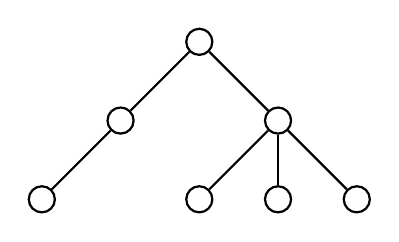
\begin{tikzpicture}[auto,
    specification/.style ={circle, draw, thick}]
   \node[specification] (A)  at (0,0)  {};
   \node[specification] (B)  at (-1,-1)  {};
   \node[specification] (C)  at (1,-1)  {};
   \node[specification] (D)  at (-2,-2)  {};
   \node[specification] (E)  at (0,-2)  {};
   \node[specification] (F)  at (1,-2)  {};
   \node[specification] (G)  at (2,-2)  {};

   \draw[thick] (A) to  (B);
   \draw[thick] (A) to (C);
   \draw[thick] (B) to (D);
   \draw[thick] (C) to (E);
   \draw[thick] (C) to (F);
   \draw[thick] (C) to (G);   
 \end{tikzpicture}
\end{minipage}
\end{frame}

\begin{frame}
    \begin{Thm}
  设树$T$有$p$个顶点,$q$条边,则$q = p-1$。
  \end{Thm}
\centering
  \begin{minipage}{0.24\linewidth}
    \centering
    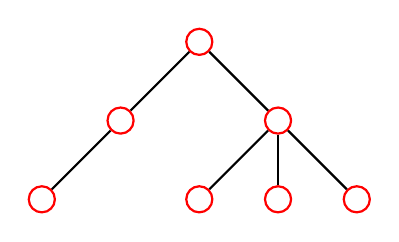
\begin{tikzpicture}[auto,
    specification/.style ={circle, draw, thick}]
   \node[specification,red] (A)  at (0,0)  {};
   \node[specification,red] (B)  at (-1,-1)  {};
   \node[specification,red] (C)  at (1,-1)  {};
   \node[specification,red] (D)  at (-2,-2)  {};
   \node[specification,red] (E)  at (0,-2)  {};
   \node[specification,red] (F)  at (1,-2)  {};
   \node[specification,red] (G)  at (2,-2)  {};

   \draw[thick] (A) to  (B);
   \draw[thick] (A) to (C);
   \draw[thick] (B) to (D);
   \draw[thick] (C) to (E);
   \draw[thick] (C) to (F);
   \draw[thick] (C) to (G);   
 \end{tikzpicture}
\end{minipage}
\end{frame}

\begin{frame}
    \begin{Thm}
  设树$T$有$p$个顶点,$q$条边,则$q = p-1$。
  \end{Thm}
\centering
  \begin{minipage}{0.24\linewidth}
    \centering
    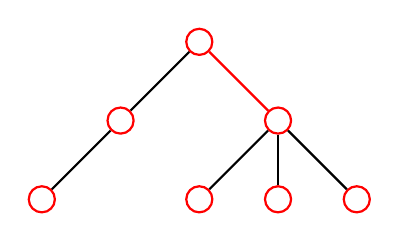
\begin{tikzpicture}[auto,
    specification/.style ={circle, draw, thick}]
   \node[specification,red] (A)  at (0,0)  {};
   \node[specification,red] (B)  at (-1,-1)  {};
   \node[specification,red] (C)  at (1,-1)  {};
   \node[specification,red] (D)  at (-2,-2)  {};
   \node[specification,red] (E)  at (0,-2)  {};
   \node[specification,red] (F)  at (1,-2)  {};
   \node[specification,red] (G)  at (2,-2)  {};

   \draw[thick] (A) to  (B);
   \draw[thick,red] (A) to (C);
   \draw[thick] (B) to (D);
   \draw[thick] (C) to (E);
   \draw[thick] (C) to (F);
   \draw[thick] (C) to (G);   
 \end{tikzpicture}
\end{minipage}
\end{frame}

\begin{frame}
    \begin{Thm}
  设树$T$有$p$个顶点,$q$条边,则$q = p-1$。
  \end{Thm}
\centering
  \begin{minipage}{0.24\linewidth}
    \centering
    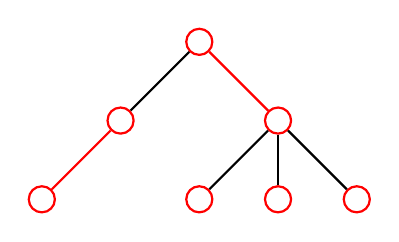
\begin{tikzpicture}[auto,
    specification/.style ={circle, draw, thick}]
   \node[specification,red] (A)  at (0,0)  {};
   \node[specification,red] (B)  at (-1,-1)  {};
   \node[specification,red] (C)  at (1,-1)  {};
   \node[specification,red] (D)  at (-2,-2)  {};
   \node[specification,red] (E)  at (0,-2)  {};
   \node[specification,red] (F)  at (1,-2)  {};
   \node[specification,red] (G)  at (2,-2)  {};

   \draw[thick] (A) to  (B);
   \draw[thick,red] (A) to (C);
   \draw[thick,red] (B) to (D);
   \draw[thick] (C) to (E);
   \draw[thick] (C) to (F);
   \draw[thick] (C) to (G);   
 \end{tikzpicture}
\end{minipage}
\end{frame}

\begin{frame}
    \begin{Thm}
  设树$T$有$p$个顶点,$q$条边,则$q = p-1$。
  \end{Thm}
\centering
  \begin{minipage}{0.24\linewidth}
    \centering
    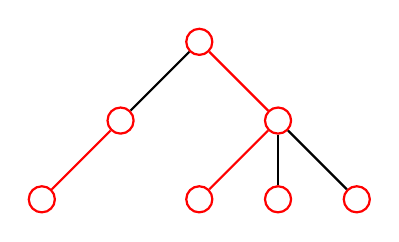
\begin{tikzpicture}[auto,
    specification/.style ={circle, draw, thick}]
   \node[specification,red] (A)  at (0,0)  {};
   \node[specification,red] (B)  at (-1,-1)  {};
   \node[specification,red] (C)  at (1,-1)  {};
   \node[specification,red] (D)  at (-2,-2)  {};
   \node[specification,red] (E)  at (0,-2)  {};
   \node[specification,red] (F)  at (1,-2)  {};
   \node[specification,red] (G)  at (2,-2)  {};

   \draw[thick] (A) to  (B);
   \draw[thick,red] (A) to (C);
   \draw[thick,red] (B) to (D);
   \draw[thick,red] (C) to (E);
   \draw[thick] (C) to (F);
   \draw[thick] (C) to (G);   
 \end{tikzpicture}
\end{minipage}
\end{frame}

\begin{frame}
    \begin{Thm}
  设树$T$有$p$个顶点,$q$条边,则$q = p-1$。
  \end{Thm}
\centering
  \begin{minipage}{0.24\linewidth}
    \centering
    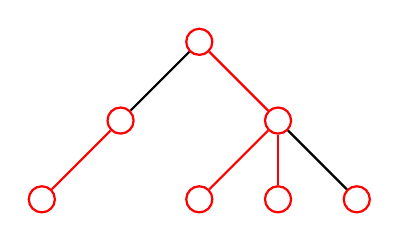
\begin{tikzpicture}[auto,
    specification/.style ={circle, draw, thick}]
   \node[specification,red] (A)  at (0,0)  {};
   \node[specification,red] (B)  at (-1,-1)  {};
   \node[specification,red] (C)  at (1,-1)  {};
   \node[specification,red] (D)  at (-2,-2)  {};
   \node[specification,red] (E)  at (0,-2)  {};
   \node[specification,red] (F)  at (1,-2)  {};
   \node[specification,red] (G)  at (2,-2)  {};

   \draw[thick] (A) to  (B);
   \draw[thick,red] (A) to (C);
   \draw[thick,red] (B) to (D);
   \draw[thick,red] (C) to (E);
   \draw[thick,red] (C) to (F);
   \draw[thick] (C) to (G);   
 \end{tikzpicture}
\end{minipage}
\end{frame}

\begin{frame}
    \begin{Thm}
  设树$T$有$p$个顶点,$q$条边,则$q = p-1$。
  \end{Thm}
\centering
  \begin{minipage}{0.24\linewidth}
    \centering
    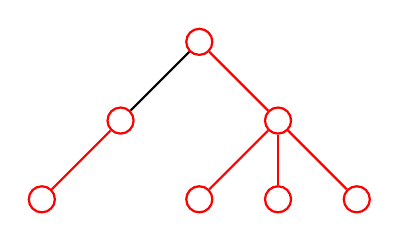
\begin{tikzpicture}[auto,
    specification/.style ={circle, draw, thick}]
   \node[specification,red] (A)  at (0,0)  {};
   \node[specification,red] (B)  at (-1,-1)  {};
   \node[specification,red] (C)  at (1,-1)  {};
   \node[specification,red] (D)  at (-2,-2)  {};
   \node[specification,red] (E)  at (0,-2)  {};
   \node[specification,red] (F)  at (1,-2)  {};
   \node[specification,red] (G)  at (2,-2)  {};

   \draw[thick] (A) to  (B);
   \draw[thick,red] (A) to (C);
   \draw[thick,red] (B) to (D);
   \draw[thick,red] (C) to (E);
   \draw[thick,red] (C) to (F);
   \draw[thick,red] (C) to (G);   
 \end{tikzpicture}
\end{minipage}
\end{frame}

\begin{frame}
    \begin{Thm}
  设树$T$有$p$个顶点,$q$条边,则$q = p-1$。
  \end{Thm}
\centering
  \begin{minipage}{0.24\linewidth}
    \centering
    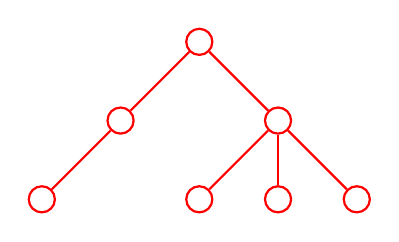
\begin{tikzpicture}[auto,
    specification/.style ={circle, draw, thick}]
   \node[specification,red] (A)  at (0,0)  {};
   \node[specification,red] (B)  at (-1,-1)  {};
   \node[specification,red] (C)  at (1,-1)  {};
   \node[specification,red] (D)  at (-2,-2)  {};
   \node[specification,red] (E)  at (0,-2)  {};
   \node[specification,red] (F)  at (1,-2)  {};
   \node[specification,red] (G)  at (2,-2)  {};

   \draw[thick,red] (A) to  (B);
   \draw[thick,red] (A) to (C);
   \draw[thick,red] (B) to (D);
   \draw[thick,red] (C) to (E);
   \draw[thick,red] (C) to (F);
   \draw[thick,red] (C) to (G);   
 \end{tikzpicture}
\end{minipage}
\end{frame}

\begin{frame}
  \begin{Thm}\small
  设树$T$有$p$个顶点,$q$条边,则$q = p-1$。
\end{Thm}\pause
  \begin{proof}[证明]\small
      用数学归纳法证明,施归纳于边数$q$。\pause
    
    (1)当$q=0$时,$p=1$,结论显然成立。\pause

    (2)假设当$q<k$时结论成立,往证当$q=k$时结论也成立。\pause 设$T$有$k$条边。\pause去掉
    $T$中的任意一条边,
    得到两个支$T_1$和$T_2$,它们均连通无圈,因此为树。\pause设$T_1$有$p_1$个顶点,
    $k_1$条边,$T_2$有$p_2$个顶点,$k_2$条边,由归纳假设,
    \begin{equation*}
      \begin{split}
        k_1 &= p_1 - 1\\
        k_2 &= p_2 - 1
      \end{split}
    \end{equation*}\pause
    以上两式相加,两边再同时加1,得
    \[k_1 + k_2  + 1 = p_1 + p_2 - 1\]
    \pause从而
    \[k = p - 1 \]
    即当$q=k$时结论也成立。
\end{proof}

\end{frame}

\begin{frame}
  \begin{Exercise}\small\justifying\let\raggedright\justifying
  设$a_1$,$a_2$,$\cdots$,$a_p$为$p$个正整数,$p\geq 2$,并且$\sum_{i=1}^pa_i=2(p-1)$。证明:存在一棵具有$p$个顶点的树,它的各个顶点的度分别为$a_1$,$a_2$,$\cdots$,$a_p$。
\end{Exercise}\pause
\begin{proof}[证明]\small\justifying\let\raggedright\justifying
  用数学归纳法证明,施归纳于$p$。\pause

  (1)当$p=2$时,$a_1+a_2=2(2-1)=2$。\pause 由$a_1$,$a_2$为正整数知,$a_1=1$,$a_2=1$。\pause两个顶点之间联结一条边,就构成了一棵满足条件的树。\pause

  (2)假设当$p=k(k\geq 2)$时结论成立,往证当$p=k+1$时结论也成立。\pause设$a_1$,$a_2$,$\cdots$,$a_{k+1}$为$k+1$个正整数,并且$\sum_{i=1}^{k+1}a_i=2(k+1-1)=2k$。\pause此时必存在$s$,$1\leq s \leq k+1$,使得$a_s=1$。\pause否则,如果对任意的$i$,$1\leq i \leq k+1$,有$a_i\geq 2$,那么$\sum_{i=1}^{k+1}a_i\geq 2(k+1)$,与$\sum_{i=1}^{k+1}a_i=2k$矛盾。\pause不妨设$a_{k+1}=1$。\pause此时必存在$t$,$1\leq t \leq k$,$a_t>1$。\pause否则,$a_1=a_2=\cdots=a_k=1$,于是$\sum_{i=1}^{k+1}a_i=k+1<2k$,矛盾。\pause不妨设$a_k>1$。\pause于是$a_1,a_2,\cdots,a_{k-1},a_{k}-1$为正整数,并且$a_1 + a_2 + \cdots + a_{k-1} + (a_{k}-1) = 2(k-1)$。\pause由归纳假设,存在一棵具有$k$个顶点的树,它的各个顶点的度分别为$a_1$,$a_2$,$\cdots$,$a_{k-1}$,$a_k-1$。\pause 在其度为$a_k-1$的顶点上联结一条边和一个顶点,便得到了一棵具有$k+1$个顶点的树,它的各个顶点的度分别为$a_1$,$a_2$,$\cdots$,$a_{k+1}$。
\end{proof}
\end{frame}
\begin{frame}
  \begin{minipage}{0.3\linewidth}
    241131211\pause

    24113111\pause

    2411211\pause

    241111\pause

    23111\pause

    2211\pause

    211\pause

    11\pause
  \end{minipage}
    \begin{minipage}{0.5\linewidth}
    \centering
    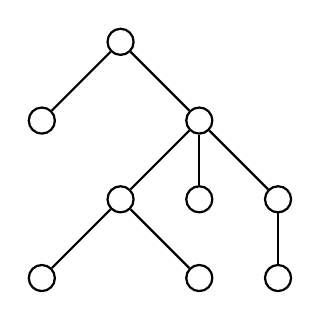
\begin{tikzpicture}[auto,
    specification/.style ={circle, draw, thick}]
   \node[specification] (A)  at (-1,-1)  {};
   \node[specification] (B)  at (0,0)  {};
   \draw[thick] (A) to  (B);\pause
   \node[specification] (C)  at (1,-1)  {};
   \draw[thick] (B) to  (C);\pause
   \node[specification] (D)  at (0,-2)  {};
   \draw[thick] (C) to  (D);\pause
   \node[specification] (E)  at (1,-2)  {};
   \draw[thick] (C) to  (E);\pause
   \node[specification] (F)  at (2,-2)  {};
   \draw[thick] (C) to  (F);\pause
   \node[specification] (G)  at (-1,-3)  {};
   \draw[thick] (D) to  (G);\pause
   \node[specification] (H)  at (1,-3)  {};
   \draw[thick] (D) to  (H);\pause
   \node[specification] (I)  at (2,-3)  {};
   \draw[thick] (F) to  (I);
 \end{tikzpicture}
\end{minipage}

\end{frame}
\end{CJK*}
\end{document}
